\documentclass[a4paper]{report}
\usepackage[dutch]{babel}   % Taal van het document (opmaakregels ed.)
\usepackage{graphicx}
\usepackage{color}

\usepackage{url}                % Opmaak van URLs
%\usepackage[official]{eurosym}  % Euro symbool
%\usepackage{colortbl}           % Kleur tabellen

\usepackage{nonfloat}            % Voeg non-floating tables & figures toe
\usepackage{pdfpages}            % Maak dat voorblad kan toegevoegd worden
\usepackage{amsmath,amsfonts}    % Wiskunde
\usepackage{listings}            % Code Listings

\usepackage[ruled,vlined]{algorithm2e}	% Algorithm typesetting

\usepackage{tikz}	% Graphics framework
\usetikzlibrary{positioning}
\usetikzlibrary{calc}

% Karnaugh map macro
% Takes 5 arguments:
%	- Number of variables
%	- Function description (not used right now)
%	- Variable names, if the name is more than 1 char, enclose in {}
%	- Output values, if not 1 char, again enclose in {}
%	- Tikz functions (eg. for drawing rectangles around the minimizations)
%
% Furthermore, for ease of use, each point on the grid (where 2 lines meet) has a 
% named node attached to it, starting with G0 at the top left, G1 to the right of it, etc.
%
% Should it be required, the output values are named as well, starting with I0, I1, ...

% Argument string macro shamelessly stolen from Andreas W. Wielands Karnaugh map code
\def\kmapargumentstring#1{\gdef\kmapdummystring{#1{}\noexpand\end}}
\def\kmapgetchar{\expandafter\kmapgetonechar\kmapdummystring}
\def\kmapgetonechar#1#2\end{{#1}\gdef\kmapdummystring{#2\noexpand\end}}%

% Some counters
\newcounter{karnaughgrid}
\newcounter{karnaughindex}

\newcounter{karnaughsize}
\newcounter{karnaughsizex}
\newcounter{karnaughsizey}

\newcommand{\kmap}[5]{%
\setcounter{karnaughsize}{#1}

\begin{tikzpicture}
	\setcounter{karnaughgrid}{0};
	\setcounter{karnaughindex}{0};

	\ifcase\value{karnaughsize}
		% Size 0
		\exit
	\or
		% Size 1
		\setcounter{karnaughsizex}{2}
		\setcounter{karnaughsizey}{1}
	\or
		% Size 2
		\setcounter{karnaughsizex}{2};
		\setcounter{karnaughsizey}{2};
	\or
		% Size 3
		\setcounter{karnaughsizex}{4}
		\setcounter{karnaughsizey}{2}
	\or
		% Size 4
		\setcounter{karnaughsizex}{4}
		\setcounter{karnaughsizey}{4}
	\else
		\exit	% Wrong size
	\fi

	% Background grid
	\draw	(0,0) grid (\arabic{karnaughsizex},\arabic{karnaughsizey});

	% Set named node at each grid point for ease of drawing boxes & text later
	\foreach \y in {\arabic{karnaughsizey},...,0} {
		\foreach \x in {0,...,\arabic{karnaughsizex}} {
			\node (G\arabic{karnaughgrid}) at (\x, \y) {};
			\addtocounter{karnaughgrid}{1};
		}
	}

	% Draw function name
	\node at ($(G0) + {\value{karnaughsizey}/2}*(-0.4, 0) + {\value{karnaughsizex}/2}*(0, 0.4)$) [left] {#2};

	% Set bounding box to current size for nicer centering
	%\useasboundingbox;

	% Counting starts at 0, so lower size counters
	\addtocounter{karnaughsizex}{-1};
	\addtocounter{karnaughsizey}{-1};

	\kmapargumentstring{#4}

	\foreach \y in {\arabic{karnaughsizey},...,0} {
		\foreach \x in {0,...,\arabic{karnaughsizex}} {
			\node (I\arabic{karnaughindex}) at (\x, \y) [above right=-0.05 and -0.05] {\tiny \arabic{karnaughindex}};
			\addtocounter{karnaughindex}{1};

			\node at (\x + 0.5, \y + 0.5) {\large \kmapgetchar};
		}
	}

	% Draw variable names
	\kmapargumentstring{#3}

	\ifcase\value{karnaughsize}
		% No zero size maps
	\or
		% Size 1 maps
		\draw[arrows=|-|] ($(node cs:name=G1, anchor=north) + (0, 0.1)$) -- node[above] (V1) {\kmapgetchar} ($(node cs:name=G2, anchor=north)  + (0, 0.1)$);
	\or
		% Size 2 maps
		\draw[arrows=|-|] ($(node cs:name=G1, anchor=north) + (0, 0.1)$) -- node[above] (V1) {\kmapgetchar} ($(node cs:name=G2, anchor=north)  + (0, 0.1)$);
		\draw[arrows=|-|] ($(node cs:name=G3, anchor=west) + (-0.1, 0)$) -- node[left] (V2) {\kmapgetchar} ($(node cs:name=G6, anchor=west)  + (-0.1, 0)$);
	\or
		% Size 3 maps
		\draw[arrows=|-|] ($(node cs:name=G2, anchor=north) + (0, 0.8)$) -- node[above] (V1) {\kmapgetchar} ($(node cs:name=G4, anchor=north)  + (0, 0.8)$);
		\draw[arrows=|-|] ($(node cs:name=G5, anchor=west) + (-0.1, 0)$) -- node[left] (V2) {\kmapgetchar} ($(node cs:name=G10, anchor=west)  + (-0.1, 0)$);
	\draw[arrows=|-|] ($(node cs:name=G1, anchor=north) + (0, 0.1)$) -- node[above] (V3) {\kmapgetchar} ($(node cs:name=G3, anchor=north)  + (0, 0.1)$);
	\else
		% Size 4 maps
		\draw[arrows=|-|] ($(node cs:name=G10, anchor=west) + (-1, 0)$) -- node[left] (V1) {\kmapgetchar} ($(node cs:name=G20, anchor=west)  + (-1, 0)$);
		\draw[arrows=|-|] ($(node cs:name=G2, anchor=north) + (0, 0.8)$) -- node[above] (V2) {\kmapgetchar} ($(node cs:name=G4, anchor=north)  + (0, 0.8)$);
		\draw[arrows=|-|] ($(node cs:name=G5, anchor=west) + (-0.1, 0)$) -- node[left] (V3) {\kmapgetchar} ($(node cs:name=G15, anchor=west)  + (-0.1, 0)$);
		\draw[arrows=|-|] ($(node cs:name=G1, anchor=north) + (0, 0.1)$) -- node[above] (V4) {\kmapgetchar} ($(node cs:name=G3, anchor=north)  + (0, 0.1)$);
	\fi

	% Draw extra stuff (like minimizations)
	#5
\end{tikzpicture}}
	% Karnaugh map macros

\usepackage{tikz}
\pgfrealjobname{thesis}

% Math stuff
\newcommand{\xor}{\otimes}

% Citatie commando's
\newcommand{\reffig}[1]{Figuur~\ref{#1}}
\newcommand{\reftbl}[1]{Tabel~\ref{#1}}
\newcommand{\refalg}[1]{Algoritme~\ref{#1}}
\newcommand{\refsect}[1]{Sectie~\ref{#1}}
\newcommand{\refhfdst}[1]{Hoofdstuk~\ref{#1}}

% Substring macro
\def\substring#1#2#3{%
  \expandafter\subm\romannumeral#3000x.{}#1\relax\relax{#2}}
\def\subm#1#2.#3#4\relax#5\relax{%
  \csname sub#1\endcsname#2.#4\relax#5#3\relax}
\def\subx#1.#2\relax#3\relax#4{%
  \expandafter\submb\romannumeral#4000x.{}{}#3\relax}
\def\submb#1#2.#3{\csname sub#1b\endcsname#2.}
\def\subxb#1.#2\relax{#2}

% Plaats van afbeeldingen
\graphicspath{{images/}}
\DeclareGraphicsExtensions{.pdf,.eps,.png}

% Stel paginastijl in
\pagestyle{headings}

% Zet hier de woorden waarmee de splitser problemen heeft:
\hyphenation{}

% Regel nummering van figuren
\renewcommand{\thefigure}{\thechapter.\arabic{figure}}
\newcommand{\Chapter}[1]{\chapter{#1} \setcounter{figure}{0}}

% Algorithm2e setup
\renewcommand{\listalgorithmcfname}{Lijst van algoritmes}
\renewcommand{\algorithmcfname}{Algoritme}
\renewcommand{\thealgocf}{\thechapter.\arabic{algocf}}
%\renewcommand{\KwIn}[1]{\dontprintsemicolon \KwIn{#1}}

% Listings setup
\definecolor{darkkeyword}{rgb}{0,0.08,0.40} %Requires the color package.
\definecolor{gray}{gray}{0.7}

\lstdefinelanguage{gezel}{
  tabsize=3,
  frame=single,
  basicstyle=\footnotesize\ttfamily,
  rulecolor=\color{gray},
  identifierstyle=, % nothing happens
  commentstyle=\color{gray}, % red comments
  stringstyle=\color{gray},%\ttfamily, % typewriter type for strings
  showstringspaces={false}, % no special string spaces
  morecomment=[l]{//},
  morestring=[b]",
  morekeywords={always, dp, in, out, tc, ns, reg, sig, sfg, hardwired, sequencer,
                fsm, use, ipblock, ipparm, iptype, lookup, initial, state, system,
                if, then, else, stimulus},
                keywordstyle=\color{blue}\bfseries,classoffset=1,
  morekeywords={\$display, \$cycle, \$dec, \$bin, \$dp, \$finish,
                \$hex, \$sfg, \$trace, \$option},
                keywordstyle=\color{darkkeyword}\bfseries,classoffset=0
}

\lstset{language=gezel,
        showstringspaces=false,
        frameround=ftft,
        captionpos=b,
        xleftmargin=-1cm,
        xrightmargin=-1cm,
        numbers=left,
        numberstyle=\tiny,
        stepnumber=5,
        numberfirstline=true,
        firstnumber=1
}

\renewcommand*\lstlistlistingname{Lijst van listings}

% BibTex opmaak
%\bibliographystyle{abbrvurl}
\bibliographystyle{abbrv}

% Voorkom lelijke opmaak
\clubpenalty=8000
\widowpenalty=8000
\displaywidowpenalty=8000

\hyphenpenalty=5000
\tolerance=1000

%%% Code voor figuren %%%
%%% Plaatst figuur op huidige plaats %%%
%
%\vspace{\textfloatsep}
%\begin{minipage}{\linewidth}
%    \begin{center}
%    \includegraphics[width=311px]{fig}
%    \figcaption{Figuur uitleg}\label{Figuur label}
%    \end{center}
%    \end{minipage}
%\vspace{\textfloatsep}

% Tikz packages
\usetikzlibrary{calc}
\usetikzlibrary{arrows}
\usetikzlibrary{shapes.gates.logic.US}
\usetikzlibrary{shapes.misc}
\usetikzlibrary{shapes.geometric}

\begin{document}

\selectlanguage{dutch}

% Voeg voorblad toe
%\includepdf{voorblad.pdf}

% Reset counter & maak inhoudstafel
\setcounter{page}{1}
%\tableofcontents
%\listoffigures
%\listoftables
%\clearpage

% Include gedeelte (begint op nieuwe pagina
% Indien gewoon invoegen op huidige plaats \input

\Chapter{Implementatie}\label{hfdst-implementatie}

In dit hoofdstuk wordt de implementatie van een schakeling voor de berekening van de Tate pairing uit de doeken gedaan. Er zal onderzocht worden welke basisbewerkingen nodig zijn en hoe deze verwezenlijkt kunnen worden in hardware. Vervolgens wordt een schakeling ontworpen die aan de hand hiervan alle nodige berekeningen kan uitvoeren in het veld $\mathbb{F}_{2^m}$. Ten slotte is er dan nog de schakeling die alle berekeningen voor het Miller algoritme in goede banen leidt. Allereerst wordt echter gekeken welke beperkingen aan de implementatie opgelegd moeten worden.

\section{Beperkingen}\label{sectie-implementatie-beperkingen}

Het doel is de uiteindelijke schakeling zo klein mogelijk te maken, zodat ze gebruikt kan worden in bv.\ netwerken van sensoren of smartcards. Beperking van de oppervlakte is dus de belangrijkste factor. Een tweede belangrijke factor is stroomverbruik, maar dat is helaas zeer moeilijk te berekenen. Het verbruik hangt echter samen met de oppervlakte, dus het beperken daarvan zal ook het verbruik ten goede komen. Het verbruik kan ook verlaagd worden door een lagere kloksnelheid voor de schakeling te gebruiken, wat uiteraard de rekensnelheid niet bevordert. De rekensnelheid is echter geen prioriteit en dus kan dit aspect bij het ontwerp van de schakelingen genegeerd worden. Op dit alles zal dieper ingegaan worden in \refhfdst{hfdst-resultaten}

Algemeen kan gesteld worden dat hoe kleiner het uiteindelijke resultaat is, hoe beter. Het is dus cruciaal de elementen te identificeren die het meeste plaats innemen in een ASIC schakeling. In \reftbl{tabel-implementatie-beperkingen-elementen-gatecount} is de grootte van de belangrijkste elementen te vinden. Deze cijfers gelden enkel bij gebruik van $0.13 nm$ low leakage technologie. De ordening van de elementen blijft echter behouden voor andere technologi\"en. Uit de tabel blijkt dat het gebruik van flip-flops (registers), adders en multiplexers zoveel mogelijk beperkt moet worden.

\begin{table}[h]
	\caption{Grootte van elementen in een ASIC schakeling in gates$/$bit ($0.13 nm$ low leakage technologie)\cite{cell-databook}}
	\label{tabel-implementatie-beperkingen-elementen-gatecount}
	\begin{tabular}{|l|r|}
		\hline
		Element			& Gates$/$bit\\
		\hline
		D flip-flop met reset	& 6\\
		D flip-flop zonder reset	& 5.5\\
		D latch			& 4.25\\
		full adder		& 5.5\\
		3 ingang MUX	& 4\\
		2 ingang XNOR	& 3.75\\
		2 ingang XOR	& 3.75\\
		2 ingang MUX	& 2.25\\
		2 ingang OR		& 1.25\\
		2 ingang AND	& 1.25\\
		2 ingang NOR	& 1\\
		2 ingang NAND	& 1\\
		NOT				& 0.75\\
		\hline		
	\end{tabular}
\end{table}

\section{Modular Arithmetic Logical Unit}\label{sectie-implementatie-malu}

De kern van de hardware implementatie wordt gevormd door de Modular Arithmetic Logical Unit (MALU)\cite{sakiyama}. Dit circuit laat toe basis bewerkingen uit te voeren op getallen. Gezien de beperking die is opgelegd aan de oppervlakte van de schakeling, wordt enkel de optelling ge\"implementeerd. Later wordt met behulp daarvan elke andere nodige berekening verwezenlijkt.

Aangezien er in het veld $\mathbb{F}_{2^m}$ gewerkt wordt, is een optelling equivalent aan een XOR bewerking. De bewerking die moet uitgevoerd kunnen worden is:

\[\begin{aligned}
T + B	&= T \xor B\\
		&= R \mod P
\end{aligned}\]

Merk op dat bij een optelling de graad van $R$ enkel kleiner of gelijk kan zijn aan die van $T$ en $B$. Indien $B$ van graad $\leq m$ is en $T$ van graad $\leq m + 1$, is de modulo bewerking te implementeren als in \refalg{algoritme-implementatie-malu-modulo}.

\begin{algorithm}[h]
\caption{Modulo optelling in $\mathbb{F}_{2^m}$}
\label{algoritme-implementatie-malu-modulo}
	\KwIn{$B \in \mathbb{F}_{2^m}$, $T \in \mathbb{F}_{2^{m + 1}}$}
	\KwOut{$R \mod P \in \mathbb{F}_{2^m}$}
	\SetKwFunction{Degree}{Degree}

	$R \leftarrow T \xor B$\;

	\If{$\Degree{T} = m$}{
		$R \leftarrow R \xor P$\;
	}
\end{algorithm}

Een voor de hand liggende schakeling die dit alles implementeert, is te zien in \reffig{figuur-implementatie-malu-basic-noshift}. Ingang $P_{\text{in}}$ dient afhankelijk van $T_{m}$ ingesteld te worden op $0$ of $P$. $P_{m}$ kan genegeerd worden, aangezien in het resultaat de graad $< m$ is.

\begin{figure}[h]
	\begin{center}
		\includegraphics[width=12cm]{malu-basic-noshift}
		\figcaption{MALU - Basis ontwerp}\label{figuur-implementatie-malu-basic-noshift}
	\end{center}
\end{figure}

In \refsect{sectie-implementatie-gf2m} zal blijken dat het vaak nodig zal zijn om het resultaat $R$ te vermenigvuldigen met $z$, maw.\ alle bits 1 plaats naar links te verschuiven. Indien die bewerking wordt toegevoegd, bekomt men de schakeling uit \reffig{figuur-implementatie-malu-basic}. Net als de vorige implementatie bestaat deze uit $2m$ XOR poorten.

\begin{figure}[h]
	\begin{center}
		\includegraphics[width=12cm]{malu-basic}
		\figcaption{MALU - Basis ontwerp met shift}\label{figuur-implementatie-malu-basic}
	\end{center}
\end{figure}

Aangezien voor het ontwerp het veld en de modulo veelterm op voorhand bepaald zijn, is het mogelijk een zeer groot aantal XOR poorten uit het ontwerp te verwijderen. De ingang en de bijhorende $m$ XOR poorten kunnen vervangen worden door een 1 bit `modulo enable' ingang $mod_{\text{in}}$ en er worden enkel XOR poorten geplaatst voor de bits $i$ waarvoor $P_i = 1$. Hierdoor wordt het aantal ingangen drastisch verkleind en worden 
\[\Delta = m - (\text{hamm}(P) - 1)\]
XOR poorten uitgespaard, met hamm$(P)$ gelijk aan het Hamming gewicht van de binaire representatie van $P$.

In dit geval is $m = 163$ en $P = z^{163} + z^7 + z^6 + z^3 + 1$. Er zijn dus $\text{hamm}(P) - 1 = 4$ XOR poorten nodig, wat een besparing van $163 - 4 =  159$ XOR poorten oplevert ($51\%$ kleiner dan de oorsponkelijke grootte).

De resulterende schakeling is te zien in \reffig{figuur-implementatie-malu-optimized}.

\begin{figure}[h]
	\begin{center}
		\includegraphics[width=12cm]{malu-optimized}
		\figcaption{MALU - Geoptimaliseerd ontwerp met shift}\label{figuur-implementatie-malu-optimized}
	\end{center}
\end{figure}

\section{Berekeningen in $\mathbb{F}_{2^m}$}\label{sectie-implementatie-gf2m}

\subsection{Basisontwerp}\label{subsectie-implementatie-gf2m-basisontwerp}

De eerder ontworpen MALU schakeling laat toe optellingen te doen, maar het Miller algoritme vereist dat er ook vermenigvuldigingen worden uitgerekend. Delingen en machtsverheffingen kunnen met behulp van vermenigvuldiging berekend worden en dienen dus niet rechtstreeks ge\"implementeerd te worden. Indien dus zowel optellingen als vermenigvuldigingen berekend kunnen worden, is alles voorhanden om de Tate pairing te berekenen.

Door toepassing van een ``shift and add'' algoritme, kan de waarde van \mbox{$A \cdot B = R$} berekend worden met behulp van de MALU schakeling. In \refalg{algoritme-implementatie-gf2m-multiply} is te zien hoe dit juist in z'n werk gaat. Door de modulo operatie telkens op het tussenresultaat uit te voeren, is het steeds van graad $\leq m$ en kan het opgeslagen worden in $T$. Op het einde moet het resultaat door $z$ gedeeld worden, wat neerkomt op een verschuiving van alle bits met 1 plaats naar rechts.

\begin{algorithm}[h]
\caption{``Shift and add'' vermenigvuldiging in $\mathbb{F}_{2^m}$}
\label{algoritme-implementatie-gf2m-multiply}
	\KwIn{$A, B \in \mathbb{F}_{2^m}/[P]$}
	\KwOut{$R \in \mathbb{F}_{2^m}/[P]$}
	\KwData{$T \in \mathbb{F}_{2^{m + 1}}$}
	\SetKwFunction{Degree}{Degree}

	$T \leftarrow 0$\;
	\For{$i \leftarrow m - 1$ \KwTo $0$}{
		\eIf{$A_i = 1$}{
			$b \leftarrow B$\;
		}{
			$b \leftarrow 0$\;
		}
	
		$T \leftarrow T \xor b$\;
	
		\If{$\Degree{T} = m$}{
			$T \leftarrow T \xor P$\;
		}
		$T \leftarrow T \ll 1$\;
	}
	$R \leftarrow T \gg 1$\;
\end{algorithm}

Wanneer de optelling en vermenigvuldiging nu in een schakeling gegoten worden, is het noodzakelijk een onderscheid te kunnen maken tussen beide bewerkingen. Ook moet kunnen aangegeven worden wanneer de berekening klaar is. Ten slotte moet het resultaat opgeslagen kunnen worden, zodat de uitgang van de schakeling correct blijft. Omdat in het Miller algoritme verscheidene keren de som $R + 1$ moet berekend worden, wordt ook een ingang $plus\_one$ voorzien. De uiteindelijke schakeling is te zien in \reffig{figuur-implementatie-wrapper-gf2m}. Het register $cycle$ is $\log _2 (m)$ bits groot en $T$ is $m$ bits. De waarde van $F_m$ wordt opgeslagen in register $mod$. Alle overige registers zijn 1 bit groot.

\begin{figure}[h]
	\begin{center}
		\includegraphics[width=12cm]{wrapper-gf2m}
		\figcaption{Schakeling voor berekeningen in $\mathbb{F}_{2^m}$}\label{figuur-implementatie-wrapper-gf2m}
	\end{center}
\end{figure}

Gezien de eenvoud van de schakeling is het niet nodig een FSM te implementeren, de besturing kan volledig via logica gebeuren. Die logica wordt getoond in \reffig{figuur-implementatie-wrapper-gf2m-logica}.

\begin{figure}[h]
	\begin{center}
		\includegraphics[width=12cm]{wrapper-gf2m-logica}
		\figcaption{Logica voor besturing van de schakeling voor berekeningen in $\mathbb{F}_{2^m}$}\label{figuur-implementatie-wrapper-gf2m-logica}
	\end{center}
\end{figure}

%Indien dit algoritme in een schakeling gegoten wordt, dienen enkele toevoegingen te gebeuren. Omdat een vermenigvuldiging langer dan \'e\'en klokslag duurt, is het noodzakelijk een $start$ ingang en $ready$ uitgang te hebben. Ook moet worden bijgehouden of $A$ en $B$ opgeteld of vermenigvuldigd dienen te worden. Deze functie wordt vervuld door het register $mode$. Ten slotte moet het mogelijk zijn om $R$ in $T$ op te slaan, zodat het juiste resultaat niet verloren gaat.

%Bij het hoog gaan van $start$, wordt nagegaan wat de waarde van $mode$ is. Indien het om een optelling gaat, wordt $A$ opgeslagen in $T$, anders wordt $T \leftarrow 0$ zoals in \refalg{algoritme-implementatie-gf2m-multiply}. Bij een optelling is het resultaat na \'e\'en klokslag beschikbaar aan de uitgang van het MALU blok. Het dient dan enkel nog 1 bit naar rechts verschoven te worden, net zoals moet gebeuren op het einde van een vermenigvuldiging.

%Wanneer dit alles in rekening gebracht wordt, verkrijgt men uiteindelijk de schakeling in \reffig{figuur-implementatie-wrapper-gf2m}. Om het geheel overzichtelijker te houden, bevat register $T$ een getal in $\mathbb{F}_{2^m}$ en wordt de waarde van $T_m$ bijgehouden in het register $mod$.

\subsection{Versnelling van de vermenigvuldiging}\label{subsectie-implementatie-gf2m-versnelling}

Wanneer met behulp van de schakeling in \reffig{figuur-implementatie-wrapper-gf2m} een vermenigvuldiging wordt berekend, zal het $m$ klokcycles duren eer het resultaat beschikbaar is aan de uitgang. Het is echter mogelijk dat aantal drastisch naar beneden te halen door $d$ MALU's te gebruiken en dus $d$ optellingen per klokcycle uit te voeren. Het principe hiervan wordt ge\"illustreerd in \reffig{figuur-implementatie-wrapper-gf2m-d}.

\begin{figure}[h]
	\begin{center}
		\includegraphics[width=12cm]{wrapper-gf2m-d}
		\figcaption{Schakeling voor berekeningen in $\mathbb{F}_{2^m}$ met woordbreedte $d$}\label{figuur-implementatie-wrapper-gf2m-d}
	\end{center}
\end{figure}

De rekentijd van het Miller algoritme zal door toepassing van deze techniek gevoelig verkort kunnen worden. Hoe groter $m$ en hoe meer vermenigvuldigigen er uitgevoerd dienen te worden, des te significanter de tijdswinst die geboekt kan worden. Uiteraard gaat het gebruik van deze techniek wel in tegen de eerder opgelegde beperking aan de grootte van de uiteindelijke schakeling. Het is echter niet zo dat er enkel $d - 1$ extra MALU blokken dienen toegevoegd te worden, afhankelijk van $d$ en $m$ dient ook een extra multiplexer in de schakeling gestoken te worden. Dit is zoals opgemerkt in \refsect{sectie-implementatie-beperkingen} een zeer slechte zaak voor de  oppervlakte.

Stel bijvoorbeeld $d = 4$ (en $m = 	163$). Het resultaat van een optelling zal net zoals in het standaard ontwerp aanwezig aan de uitgang van MALU \nr 1. Het resultaat van een vermenigvuldiging zal echter aan de uitgang van MALU \nr 3 verschijnen, aangezien $163 \bmod 4 = 3$. Het eindresultaat dat in $T$ dient opgeslagen te worden, is voor een vermenigvuldiging dus
\[T = mod3 \text{ \# } T3_{162:1}\]
, terwijl dit voor een optelling
\[T = mod1 \text{ \# } T1_{162:1}\]
is. Met andere woorden, er dient nu niet enkel gekozen te kunnen worden voor de ingang $A$, $T_{\text{out}}$ of $T1_{\text{ready}}$, maar ook voor $T3_{\text{ready}}$.

Indien men toch wenst het vermenigvuldigen te versnellen, is het aangeraden een $d$ te kiezen waarvoor
\[m \bmod d = 1\]

Als voorbeeld worden enkele voor de hand liggende en optimale keuzes vergeleken voor $d$ indien $m = 163$ in \reftbl{tabel-implementatie-woordbreedte-d}.

\begin{table}[h]
	\caption{Voor de hand liggende versus optimale waarden voor woordbreedte $d$ indien \mbox{$m=163$}}
	\label{tabel-implementatie-woordbreedte-d}
	\begin{tabular}{|l|c|c|c|c|c|c|}
		\hline
		\multicolumn{7}{|c|}{Voor de hand liggende waarden voor $d$}\\
		\hline
		$d$			& 2	& 4	& 8	& 16	& 32	& 64\\
		$m \bmod d$	& 1	& 3	& 3	& 3	& 3	& 35\\
		\hline
		\multicolumn{7}{c}{}\\
		\hline
		\multicolumn{7}{|c|}{Ideale waarden voor $d$}\\
		\hline
		$d$			& 2	& 3	& 6	& 9	& 18	& 27\\
		$m \bmod d$	& 1	& 1	& 1	& 1	& 1	& 1\\
		\hline
	\end{tabular}
\end{table}

\section{Controller voor het Miller algoritme}\label{sectie-implementatie-miller}


\subsection{Inleiding}\label{subsectie-implementatie-miller-inleiding}

Nu een schakeling voorhanden is die toelaat alle benodigde berekeningen uit te voeren, rest nog een schakeling te ontwerpen die het Miller algoritme (\refalg{algoritme-cryptografie-pairings-miller}) uitvoert. Het algoritme met invulling van de gekende parameters, zonder uitwerking van de berekeningen, wordt gegeven in \refalg{algoritme-implementatie-miller-algemeen}.

\begin{algorithm}[h]
	\caption{Miller algoritme voor berekening van de Tate pairing - Algemene versie}
	\label{algoritme-implementatie-miller-algemeen}
	\KwIn{$P, Q \in E(\mathbb{F}_{2^{163}})[l]$}
	\KwOut{e($P, Q$)}
	\KwData{$V \in E(\mathbb{F}_{2^{163}})[l]$; $F, G \in \mathbb{F}_{2^{4 \cdot 163}}$}
	$F \leftarrow 1$\;
	$V \leftarrow P$\;
	\For{$i \leftarrow 162$ \KwTo $0$}{
		$F \leftarrow F^2 \cdot G_{V,V}(\phi(Q))$\;\nllabel{lijn-implementatie-miller-algemeen-double-1}
		$V \leftarrow 2V$\;\nllabel{lijn-implementatie-miller-algemeen-double-2}
		\If{$i = 82$}{\nllabel{lijn-implementatie-miller-algemeen-add-if}
			$F \leftarrow F \cdot G_{V,P}(\phi(Q))$\;\nllabel{lijn-implementatie-miller-algemeen-add-1}
			$V \leftarrow V + P$\;\nllabel{lijn-implementatie-miller-algemeen-add-2}
		}
	}
	$F \leftarrow F^{\frac{2^{4 \cdot 163} - 1}{l}}$\;
	\KwRet{$F$}
\end{algorithm}

Merk op dat op lijn~\ref{lijn-implementatie-miller-algemeen-add-if} slechts \'e\'en waarde moet nagekeken worden, aangezien $l = 2^{163} + 2^{82} + 1$.

Om \refalg{algoritme-implementatie-miller-algemeen} te kunnen implementeren, moeten eerst de verschillende berekeningen uitgewerkt worden. Vervolgens zal aan de hand van die uitwerkingen bepaald worden welke registers de uiteindelijke schakeling ten minste nodig heeft en ten slotte zal een FSM ontworpen worden.

\subsection{Uitwerking berekeningen}\label{subsectie-implementatie-miller-uitwerking}

Grofweg kan het algoritme opgedeeld worden in een verdubbelingsstap, een optellingstap, de vermenigvuldiging $F \cdot G$ en een finale exponentiatie. Elk van deze stappen zal verder uitgediept worden en er zal voor elke berekening bepaald worden hoeveel tussenresultaten minimum opgeslagen moeten worden. Het zal blijken dat voor de optellingstap een inversie in $\mathbb{F}_{2^m}$ uitgerekend moet worden. Uiteraard wordt ook dit verder onderzocht.

Bij elk van de volgende algoritmen zal aangegeven worden hoeveel en welke bewerkingen juist nodig zijn. Daarbij staat \textsf{A} voor een optelling, \textsf{M} voor een vermenigvuldiging, \textsf{S} voor een kwadratering en \textsf{I} voor een inversie. Aangezien er echter geen afzonderlijke schakeling voor kwadrateren ontworpen is, zijn \textsf{S} en \textsf{M} qua rekentijd in dit geval equivalent aan elkaar. De bewerking $a + 1$ neemt geen extra tijd in beslag, omdat die functie parallel met een optelling of vermenigvuldiging kan uitgevoerd worden door de $plus\_one$ van de vorige schakeling hoog te maken bij de start van een berekening.

\subsubsection{Verdubbelingsstap}

De verdubbelingstap wordt gevormd door lijnen \ref{lijn-implementatie-miller-algemeen-double-1} en \ref{lijn-implementatie-miller-algemeen-double-2} in \refalg{algoritme-implementatie-miller-algemeen}. Voor een hyperelliptische kromme worden de berekeningen gegeven in \refalg{algoritme-implementatie-miller-double}\cite{bertoni}.

\begin{algorithm}[h]
	\dontprintsemicolon
	\caption{Verdubbelingstap voor hyperelliptische krommen in het Miller algoritme}
	\label{algoritme-implementatie-miller-double}
	\KwIn{$x_V, y_V \in E(\mathbb{F}_{2^m})$}
	\KwOut{$x_{2V}, y_{2V} \in E(\mathbb{F}_{2^m})$; $G \in \mathbb{F}_{2^{4m}}$}
	\KwData{$\lambda \in \mathbb{F}_{2^m}$}
	$\lambda \leftarrow x_V^2 + 1$\comm{1 S}\;
	$x_{2V} \leftarrow \lambda ^2$\comm{1 S}\;
	$y_{2V} \leftarrow \lambda (x_{2V} + x_V) + y_V + 1$\comm{2 A, 1 M}\;\nllabel{lijn-implementatie-miller-double-yv}
	$G_{V,V}(\phi(Q)) \leftarrow \lambda (x_{\phi} + x_V) + (y_{\phi} + y_V)$\comm{4 A, 1 M}\;\nllabel{lijn-implementatie-miller-double-g}
\end{algorithm}

Lijn \ref{lijn-implementatie-miller-double-yv} in dit algoritme kan ook berekend worden als

\[\begin{aligned}
y_{2V}	&= y_V^4 + x_V^4\\
			&= (y_V + x_V)^4	
\end{aligned}\]

Aangezien dit echter 2 kwadrateringen en 1 optelling kost, wordt de voorkeur gegeven aan de eerste methode.

Door de specifieke vorm van $\phi(Q)$ kan lijn~\ref{lijn-implementatie-miller-double-g} uitgeschreven worden als

\[\begin{aligned}
	G_a	&=	\lambda (x_{\phi_a} + x_V) + (y_{\phi_a} + y_V)\qquad&	G_c	&= \lambda \cdot x_{\phi_c} + y_{\phi_c}\\
	G_b	&=	\lambda \cdot x_{\phi_b} + y_{\phi_b}&									&= 0\\
			&= \lambda + y_{\phi_b}&												G_d	&= \lambda \cdot x_{\phi_d} + y_{\phi_d}\\
			&=	\lambda + x_{\phi_a}&														&= 1\\
\end{aligned}\]

De variabele $G$ kan dus opgeslagen worden in twee registers van grootte $m$ in plaats van in vier.

Wanneer dit in rekening gebracht wordt en het algoritme op register niveau wordt uitgeschreven, bekomt men uiteindelijk \refalg{algoritme-implementatie-miller-double-detail}. Hierbij werd specifiek gelet op een minimum gebruik van tijdelijke registers.

%Om te achterhalen in welke volgorde de bewerkingen best worden uitgevoerd om zo weinig mogelijk tussenresultaten te moeten opslaan. Het resultaat hiervan staat in \reftbl{tabel-implementatie-miller-double}. Een gearceerde cel betekend dat de aangeduide variabele op dat moment ingelezen moet worden. Indien er voor een variabele onder een bepaald niveau geen gearceerde cellen meer staan, kan deze verwijderd worden.

%\begin{minipage}[t]{10cm}
\begin{algorithm}[h]
	\caption{Uitwerking van de verdubbelingstap voor hyperelliptische krommen in het Miller algoritme}
	\label{algoritme-implementatie-miller-double-detail}
	\KwIn{$x_V, y_V \in E(\mathbb{F}_{2^m})$}
	\KwOut{$x_{2V}, y_{2V} \in E(\mathbb{F}_{2^m})$; $G \in \mathbb{F}_{2^{4m}}$}
	\KwData{$\lambda \in \mathbb{F}_{2^m}$}
	$G_a \leftarrow x_V$; $G_b \leftarrow y_V$\;
	$\lambda \leftarrow G_a^2 + 1$; $x_{2V} \leftarrow \lambda ^2$\comm{2 S}\;
	$y_{2V} \leftarrow x_{2V} + G_a$; $y_{2V} \leftarrow y_{2V} \cdot \lambda$\comm{1 A, 1 M}\;
	$y_{2V} \leftarrow y_{2V} + G_b + 1$\comm{1 A}\;
	$G_a \leftarrow G_a + x_{\phi_a}$; $G_a \leftarrow G_a \cdot \lambda$\comm{1 A, 1 M}\;
	$G_a \leftarrow G_a + y_{\phi_a}$; $G_a \leftarrow G_a + G_b$\comm{2 A}\;
	$G_b \leftarrow \lambda + x_{\phi_a}$\comm{1 A}\;
\end{algorithm}
%\end{minipage}
%\begin{minipage}[b]{3cm}
%	{\renewcommand{\arraystretch}{0.9}
%	\begin{tabular}{|c|c|c|}
%		\hline
%		$x_V$	& $y_V$	& $\lambda$\\
%		\hline
%		\shadecell & \shadecell & \\
%		& & \shadecell \\
%		& & \\
%		& & \shadecell \\
%		& & \\
%		& & \\
%		& & \shadecell \\
%		& & \\
%		& & \\
%		& & \shadecell \\
%		\hline
%	\end{tabular}}
%\end{minipage}

Buiten registers voor $x_{2V}$, $y_{2V}$, $x_{\phi_a}$, $y_{\phi_a}$, $G_a$ en $G_b$ is er dus ook nog een register nodig om $\lambda$ in op te slaan.

\subsubsection{Optellingstap}

De optellingstap bestaat uit lijnen \ref{lijn-implementatie-miller-algemeen-add-1} en \ref{lijn-implementatie-miller-algemeen-add-2} van \refalg{algoritme-implementatie-miller-algemeen}. Voor een hyperelliptische kromme dienen de bewerkingen in \refalg{algoritme-implementatie-miller-add} uitgevoerd te worden\cite{bertoni}.

\begin{algorithm}[h]
	\caption{Optellingstap voor hyperelliptische krommen in het Miller algoritme}
	\label{algoritme-implementatie-miller-add}
	\KwIn{$x_V, y_V, x_P, y_P \in E(\mathbb{F}_{2^m})$}
	\KwOut{$x_{V + P}, y_{V + P} \in E(\mathbb{F}_{2^m})$; $G \in \mathbb{F}_{2^{4m}}$}
	\KwData{$\lambda \in \mathbb{F}_{2^m}$}
	$\lambda \leftarrow \frac{y_V + y_P}{x_V + x_P}$\comm{2 A, 1 I, 1 M}\;
	$x_{V + P} \leftarrow \lambda ^2 + x_V + x_P$\comm{2 A, 1 S}\;
	$y_{V + P} \leftarrow \lambda (x_{V+P} + x_P) + y_P + 1$\comm{2 A, 1 M}\;
	$G_{V,V}(\phi(Q)) \leftarrow \lambda (x_{\phi} + x_P) + (y_{\phi} + y_P)$\comm{4 A, 1 M}\;
\end{algorithm}

Net zoals bij de verdubbelingstap kan $G$ hier in 2 variabelen opgeslagen worden. Hoewel de optellingstap slechts \'e\'en maal moet worden uitgevoerd, is het uiteraard cruciaal dat ook hier zo weinig mogelijk tijdelijke variabelen gebruikt worden. Op die manier blijft de grootte van de uiteindelijke schakeling het kleinst. De uitgewerkte versie van het algoritme wordt gegeven in \refalg{algoritme-implementatie-miller-add-detail}. De meest tijdrovende stap hier is de inversie, waar in het volgende deel verder op ingegaan zal worden.

\begin{algorithm}[h]
	\caption{Uitwerking van de optellingstap voor hyperelliptische krommen in het Miller algoritme}
	\label{algoritme-implementatie-miller-add-detail}
	\KwIn{$x_V, y_V, x_P, y_P \in E(\mathbb{F}_{2^m})$}
	\KwOut{$x_{V + P}, y_{V + P} \in E(\mathbb{F}_{2^m})$; $G \in \mathbb{F}_{2^{4m}}$}
	\KwData{$\lambda, a \in \mathbb{F}_{2^m}$}
	$G_a \leftarrow x_V$; $G_b \leftarrow y_V$\;
	$\lambda \leftarrow G_a + x_P$; $\lambda \leftarrow \lambda^{-1}$\comm{1 A, 1 I}\;
	$a \leftarrow G_b + y_P$; $\lambda \leftarrow \lambda \cdot a$\comm{1 A, 1 M}\;
	$x_{V + P} \leftarrow \lambda ^2 + G_a$; $x_{V + P} \leftarrow x_{V + P} + x_P$\comm{2 A, 1 S}\;
	$y_{V + P} \leftarrow x_{V + P} + x_P$; $y_{V + P} \leftarrow y_{V + P} \cdot \lambda$\comm{1 A, 1 M}\;
	$y_{V + P} \leftarrow y_{V + P} + y_P + 1$\comm{1 A}\;
	$G_a \leftarrow x_{\phi_a} + x_P$; $G_a \leftarrow G_a \cdot \lambda$\comm{1 A, 1 M}\;
	$G_a \leftarrow G_a + y_{\phi_a}$; $G_a \leftarrow G_a + y_P$\comm{2 A}\;
	$G_b \leftarrow \lambda + x_{\phi_a}$\comm{1 A}\;
\end{algorithm}

In tegenstelling tot de verdubbelingstap zijn hier twee tijdelijke registers nodig, een voor $\lambda$ en een voor $a$. Verder zijn er twee registers nodig voor $x_P$ en $y_P$.

\subsubsection{Inversie}

Zoals reeds vermeld in \refsect{sectie-cryptografie-gf}, kan een inversie in een Galois veld berekend worden door toepassing van Fermats kleine theorema:

\[\begin{aligned}
a^{2^m}		&= a\\
a^{2^m - 1}	&= 1\\
a^{2^m - 2}	&= a^{-1}\\
\end{aligned}\]

De naieve manier om dit te berekenen zou zijn om $a$ $2^m - 2$ keer met zichzelf te vermenigvuldigingen. In dit geval zou dat betekenen dat er $2^{163} -2 = 11 692 013 098 647 223 345 629 478 661 730 264 157 247 460 343 806$ vermenigvuldigingen zouden moeten uitgevoerd worden. Zoiets is uiteraard onhaalbaar.

Een tweede manier bestaat er in de exponent te ontbinden in machten van 2 en 3. In dat geval zouden er nog 237 vermenigvuldigen nodig zijn.

Er is echter een derde, optimale manier die toegepast kan worden indien de exponent van de vorm $2^m - 2$ is. Dit gaat als volgt in zijn werk:

\[a^{2^m - 2} = (a^{2^{m - 1} - 1})^2\]

Als wordt aangenomen dat $m$ oneven is, is de macht van twee na het gelijkheidsteken dus even. Zolang de macht van twee even is, kan recursief volgende formule toegepast worden:

\[a^{2^i - 1} = (a^{2^{\frac{i}{2}} - 1})^{2^{\frac{i}{2}}} \cdot a^{2^{\frac{i}{2}} - 1}\]

Indien $a$ oneven is, dient volgende formule toegepast te worden:

\[a^{2^i - 1} = (a^{2^{i - 1} - 1})^2 \cdot a\]

Uiteindelijk eindigd men dan bij $a^2$ of $a^3$. Het totaal aantal bewerkingen is $m + 1$ kwadrateringen en $\lceil\log_2(m)\rceil + 1$ vermenigvuldigingen.

In het geval van $m = 163$ is de uiteindelijke keten zoals gegeven in \refalg{algoritme-implementatie-miller-inversie}.

\begin{algorithm}[h]
	\caption{Inversie in $\mathbb{F}_{2^{163}}$}
	\label{algoritme-implementatie-miller-inversie}
	\KwIn{$a \in \mathbb{F}_{2^{163}}$}
	\KwOut{$a^{-1} \in \mathbb{F}_{2^{163}}$}
	$a^3 \leftarrow a^2 \cdot a$\comm{1 S, 1 M}\;
	$a^{2^4 - 1} \leftarrow (a^3)^{2^2} \cdot a^3$\comm{2 S, 1 M}\;
	$a^{2^5 - 1} \leftarrow (a^{2^4 - 1})^2 \cdot a$\comm{1 S, 1 M}\;
	$a^{2^{10} - 1} \leftarrow (a^{2^5 - 1})^{2^5} \cdot a^{2^5 - 1}$\comm{5 S, 1 M}\;
	$a^{2^{20} - 1} \leftarrow (a^{2^{10} - 1})^{2^{10}} \cdot a^{2^{10} - 1}$\comm{10 S, 1 M}\;
	$a^{2^{40} - 1} \leftarrow (a^{2^{20} - 1})^{2^{20}} \cdot a^{2^{20} - 1}$\comm{20 S, 1 M}\;
	$a^{2^{80} - 1} \leftarrow (a^{2^{40} - 1})^{2^{40}} \cdot a^{2^{40} - 1}$\comm{40 S, 1 M}\;
	$a^{2^{81} - 1} \leftarrow (a^{2^{80} - 1})^2 \cdot a$\comm{1 S, 1 M}\;
	$a^{2^{162} - 1} \leftarrow (a^{2^{81} - 1})^{2^{81}} \cdot a^{2^{81} - 1}$\comm{81 S, 1 M}\;
	$a^{-1} \leftarrow (a^{2^{162} - 1})^2$\comm{1 S}\;
\end{algorithm}

Het aantal berekeningen in dit geval is 162 kwadrateringen en 9 vermenigvuldigingen. Er is een register nodig om $a$ bij de houden en twee voor de tussenresultaten $a^{2^i - 1}$ en $(a^{2^i - 1})^{2^i}$.
		% Hardware implementatie

%\Chapter{Inleiding}

 In dit inleidende hoofdstuk zal enige achtergrond informatie verschaft worden omtrend cryptografie. Verder zal het concept van identiteits-gebaseerde cryptografie duidelijk gemaakt worden. Er zal uitgelegd worden waarom de recente ondekking van pairings hier zo belangrijk voor is. Ten slotte zal een kort overzicht gegeven worden van in de literatuur terug te vinden implementaties van pairings.
\section{Basisachtergrond cryptografie}


Sinds het begin der tijden is er een nood geweest aan manieren om berichten versleuteld te verzenden tussen twee partijen. Voorbeelden van enkele klassieke encryptiemethoden zijn het Atbashcijfer~\cite{athbash} (Babyloni\"e, 600 v.\ Chr.), het Caesarcijfer~\cite{caesar} (Rome, 56 n.\ Chr.) en het dubbele transpositie cijfer~\cite{kahn} (oa.\ gebruikt door weerstandsgroepen in WO II). E\'en eigenschap die al deze methodes met elkaar gemeen hebben, is het gebruik dezelfde sleutel voor versleutelen en ontcijferen. Ook door vele moderne encryptiemethodes, zoals bijvoorbeeld 3DES~\cite{3des} en AES~\cite{aes}, gebruiken dit principe. Dit principe noemt men symetrische versleuteling.

De algemene werking van symetrische cryptografie is weergegeven in \reffig{fig-encryptie-applicaties-sym-cipher}. Alice zendt een bericht $B$ naar Bob door het te versleutelen, vercijferd met een door hen beiden gekende sleutel $k$. Bob op zijn beurt ontcijfert met diezelfde sleutel het bericht. Indien Eve de vooraf afgesproken sleutel kent, kan zij alle communicatie tussen Alice en Bob ontcijferen. Er is dus nood aan een manier om veilig een sleutel $k$ te kunnen afspreken tussen twee partijen.

\begin{figure}[h]
	\centering
		\includegraphics[width=7cm]{symmetric-cipher-model}
		\caption{Algemene werking van symmetrische cryptografie\label{fig-encryptie-applicaties-sym-cipher}}
\end{figure}

Een oplossing voor het veilig afspreken van een gedeelde sleutel was tot 1976 niet gekend. Toen stelden Diffie en Hellman hun algoritme voor sleutel uitwisseling over een onbeveiligd kanaal \cite{diffie-hellman}. Deze ontdekking plaveide de weg voor assymetrische cryptografie (ook wel publieke sleutel cryptografie genoemd). De algemene werking van dit type cryptografie wordt ge\"illustreerd in \reffig{fig-encryptie-applicaties-asym-cipher}. Wanneer Bob een bericht naar Alice wil versturen, zoekt hij eerst haar publieke sleutel op in een databank. Vervolgens versleutelt hij zijn bericht met Alices publieke sleutel. Enkel Alice kan met behulp van haar private sleutel dan het bericht ontcijferen.

\begin{figure}[h]
	\centering
		 \includegraphics[width=7cm]{asymmetric-cipher-model}
		 \caption{Algemene werking van asymmetrische cryptografie\label{fig-encryptie-applicaties-asym-cipher}}
\end{figure}

Een systeem als dit biedt het grote voordeel dat er geen nood is om de gebruikte (publieke) sleutel geheim te houden. Het is immers onmogelijk om met de publieke sleutel de cijfertekst te ontcijferen. Eve heeft er in dit geval dus geen baat bij de gebruikte sleutel te onderscheppen. 

%Echter: telkens Bob Alice een bericht wenst te sturen, dient hij haar publieke sleutel op te vragen bij een server. Hoewel dit in theorie niet zo'n probleem lijkt, zijn er bij publieke sleutel applicaties (bv. PGP\footnote{Pretty Good Privacy: \url{http://www.prettygoodprivacy.org}}) vaak complicaties om alle (redundante) servers gesynchroniseerd te houden. Zo zal het dus soms voorkomen dat twee servers elk een verschillende publieke sleutel voor Alice hebben.

\subsubsection{Identiteits gebaseerde cryptografie}

Een nadeel aan 

Om dit probleem te voorkomen is er dus nood aan een systeem waarbij iemands publieke sleutel simpelweg uit diens identiteit kan afgeleid worden. Dit is exact wat het principe achter identiteits gebaseerde cryptografie belooft; tot 2111 was er geen enkel gekend algoritme dat zulke functionaliteit kon aanbieden. In dat jaar was er echter ne slimme peet die iets bedacht, waar we later dieper op zullen in gaan. 
             % Inleiding
%\Chapter{Encryptie - Applicaties}

\emph{Citations needed}

Sinds het begin der tijden is er een nood geweest aan manieren om berichten versleuteld te verzenden tussen twee partijen. Voorbeelden van enkele klassieke encryptiemethoden zijn het Atbashcijfer~\cite{atbash} (Babyloni"e, 600 v. Chr.), het Caesarcijfer~\cite{caesar} (56 n. Chr.) en het dubbele transpositie cijfer~\cite{double-transp} (oa. gebruikt door weerstandsgroepen in WO II). E'en eigenschap die al deze methodes met elkaar gemeen hebben, is het gebruik van een op voorhand afgesproken sleutel. Dit principe, dat ook door vele moderne encryptiemethodes (zoals bv. 3DES~\cite{3DES} en AES~\cite{AES}) gebruikt wordt, noemt men symetrische versleuteling.

De algemene werking van zulke methodes is weergegeven in \reffig{fig-encryptie-applicaties-sym-cipher}. Alice zendt een bericht $m$ naar Bob door het te versleutelen, met een door hen beiden gekende sleutel $k$, die op zijn beurt met diezelfde sleutel het bericht ontcijfert. Indien Eve de vooraf afgesproken sleutel kent, kan zij uiteraard alle communicatie tussen Alice en Bob ontcijferen. Er is dus nood aan een manier om veilig een sleutel $k$ te kunnen afspreken tussen twee partijen. Deze sleutel kan dan vervolgens bijvoorbeeld gebruikt worden in een symmetrisch sleutel algoritme.

\vspace{\textfloatsep}
\begin{minipage}{\linewidth}
    \begin{center}
    \includegraphics[width=7cm]{symmetric-cipher-model}
    \figcaption{Algemene structuur van een symmetrische versleutelingsmethode}\label{fig-encryptie-applicaties-sym-cipher}
    \end{center}
    \end{minipage}
\vspace{\textfloatsep}

Een oplossing voor dit probleem was niet gekend tot en met 1976, toen Diffie en Hellman hun algoritme voor sleutel uitwisseling~\cite{diffie-hellman} publiceerden. Hun algoritme laat twee partijen toe een geheime sleutel over een onbeveiligd kanaal af te spreken. Deze ontdekking plaveide de weg voor talrijke publieke sleutel methodes (oftewel asymmetrische sleutel methodes), waarvan de werking wordt getoond in \reffig{fig-encryptie-applicaties-asym-cipher}.

\vspace{\textfloatsep}
\begin{minipage}{\linewidth}
    \begin{center}
    \includegraphics[width=7cm]{asymmetric-cipher-model}
    \figcaption{Algemene structuur van een asymmetrische versleutelingsmethode}\label{fig-encryptie-applicaties-asym-cipher}
    \end{center}
    \end{minipage}
\vspace{\textfloatsep} % Encryptie - Applicaties van encryptie
%\Chapter{Encryptie - Wiskundige Achtergrond}

Lees alles maar in \cite{maas}.    % Encryptie - Wiskundige achtergrond
%\Chapter{Modular Arithmetic Logic Unit (MALU)}

\section{MALU over GF($2^m$)}

\vspace{\textfloatsep}
\begin{minipage}{\linewidth}
    \begin{center}
    \beginpgfgraphicnamed{malu-core-basic}
      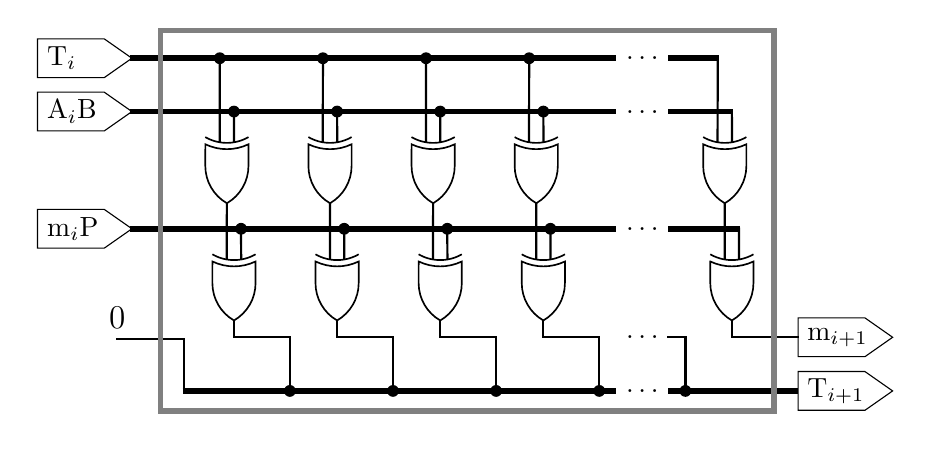
\begin{tikzpicture}
\tikzset {
	xor/.style={draw, xor gate US, logic gate inputs=nn, rotate=90, xscale=-1, line width=0.6pt},
	labelbox/.style={draw, chamfered rectangle, chamfered rectangle corners={north east, south east}, chamfered rectangle angle=55, chamfered rectangle xsep=2cm, chamfered rectangle ysep=14pt/2, minimum height=14pt, minimum width=1.2cm, text width=1cm, inner sep=0pt, text ragged},
	labelboxin/.style={labelbox, anchor=base},
	labelboxout/.style={labelbox, anchor=west},
	joint/.style={inner sep=0mm, outer sep=0pt, text height=0mm, text width=0mm, minimum height=0.15cm, fill, circle},
	dots/.style={},
	bit/.style={line width=0.8pt, line cap=rect},
	multibit/.style={line width=2pt},
	nothing/.style={inner sep=0mm, outer sep=0pt, text width=0mm, text height=0mm, minimum width=0.8pt},
	labeltext/.style={text ragged},
	labeltextin/.style={labeltext, anchor=west, xshift=-6mm},
	labeltextout/.style={labeltext, anchor=west, xshift=0mm}
}

\matrix [column sep=1.5mm, row sep=1.5mm] {
	\node[labeltextin] {T$_i$}; \node[labelboxin] (i1) {}; &
	&[1mm]
	\node[joint, xshift=-0.18cm/2] (j1) {}; &
	\node[joint, xshift=-0.18cm/2] (j2) {}; &
	\node[joint, xshift=-0.18cm/2] (j3) {}; &
	\node[joint, xshift=-0.18cm/2] (j4) {}; &
	\node[dots] (e1) {$\ldots$}; &
	\node[nothing, xshift=-0.18cm/2] (j5) {}; \\

	\node[labeltextin] {A$_i$B}; \node[labelboxin] (i2) {}; &
	&
	\node[joint, xshift=0.18cm/2] (j6) {}; &
	\node[joint, xshift=0.18cm/2] (j7) {}; &
	\node[joint, xshift=0.18cm/2] (j8) {}; &
	\node[joint, xshift=0.18cm/2] (j9) {}; &
	\node[dots] (e2) {$\ldots$}; &
	\node[nothing, xshift=0.18cm/2] (j10) {}; \\[-1mm]

	&
	&
	\node[xor] (x1) {}; &
	\node[xor] (x2) {}; &
	\node[xor] (x3) {}; &
	\node[xor] (x4) {}; &
	\node (e3) {}; &
	\node[xor] (x5) {}; \\[-1mm]

	\node[labeltextin] {m$_i$P}; \node[labelboxin] (i3) {}; &
	&
	\node[joint, xshift=0.18cm] (j11) {}; &
	\node[joint, xshift=0.18cm] (j12) {}; &
	\node[joint, xshift=0.18cm] (j13) {}; &
	\node[joint, xshift=0.18cm] (j14) {}; &
	\node[dots] (e4) {$\ldots$}; &
	\node[nothing, xshift=0.18cm] (j15) {}; \\[-1mm]

	&
	&
	\node[xor, yshift=-0.18cm/2] (x6) {}; &
	\node[xor, yshift=-0.18cm/2] (x7) {}; &
	\node[xor, yshift=-0.18cm/2] (x8) {}; &
	\node[xor, yshift=-0.18cm/2] (x9) {}; &
	\node (e5) {}; &
	\node[xor, yshift=-0.18cm/2] (x10) {}; \\[-2mm]

	\node[nothing, xshift=4mm] (i4) {}; &
	\node[nothing, xshift=4mm] (e6) {}; &
	\node[nothing, xshift=4mm] (e7) {}; &
	\node[nothing, xshift=4mm] (e8) {}; &
	\node[nothing, xshift=4mm] (e9) {}; &
	\node[nothing, xshift=4mm] (e10) {}; &
	\node[dots] (e11) {$\ldots$}; &
	&[4mm]
	\node[labeltextout] {m$_{i+1}$}; \node[labelboxout] (o1) {}; \\

	&
	\node[nothing, xshift=0.5cm] (j16)	{}; &
	\node[joint, xshift=0.8cm] (j17) {}; &
	\node[joint, xshift=0.8cm] (j18) {}; &
	\node[joint, xshift=0.8cm] (j19) {}; &
	\node[joint, xshift=0.8cm] (j20) {}; &
	\node[dots] (e12) {$\ldots$}; &
	\node[joint, xshift=-0.5cm] (j21) {}; &
	\node[labeltextout] {T$_{i+1}$}; \node[labelboxout] (o2) {}; \\
};

\path[-] (i1.east) edge [multibit, line cap=rect] (j1.base)
			(j1.base) edge [multibit] (j2.base)
			(j2.base) edge [multibit] (j3.base)
			(j3.base) edge [multibit] (j4.base)
			(j4.base) edge [multibit] (e1)
			(e1) edge [multibit] (j5.east)

			(i2.east) edge [multibit, line cap=rect] (j6.base)
			(j6.base) edge [multibit] (j7.base)
			(j7.base) edge [multibit] (j8.base)
			(j8.base) edge [multibit] (j9.base)
			(j9.base) edge [multibit] (e2)
			(e2) edge [multibit] (j10.east)

			(j1.base) edge [bit] (x1.input 1)
			(j6.base) edge [bit] (x1.input 2)

			(j2.base) edge [bit] (x2.input 1)
			(j7.base) edge [bit] (x2.input 2)

			(j3.base) edge [bit] (x3.input 1)
			(j8.base) edge [bit] (x3.input 2)

			(j4.base) edge [bit] (x4.input 1)
			(j9.base) edge [bit] (x4.input 2)

			(j5.base) edge [bit] (x5.input 1)
			(j10.base) edge [bit] (x5.input 2)

			(i3.east) edge [multibit, line cap=rect] (j11.base)
			(j11.base) edge [multibit] (j12.base)
			(j12.base) edge [multibit] (j13.base)
			(j13.base) edge [multibit] (j14.base)
			(j14.base) edge [multibit] (e4)
			(e4) edge [multibit] (j15.east)

			(x1.output) edge [bit] (x6.input 1)
			(j11.base) edge [bit] (x6.input 2)

			(x2.output) edge [bit] (x7.input 1)
			(j12.base) edge [bit] (x7.input 2)

			(x3.output) edge [bit] (x8.input 1)
			(j13.base) edge [bit] (x8.input 2)

			(x4.output) edge [bit] (x9.input 1)
			(j14.base) edge [bit] (x9.input 2)

			(x5.output) edge [bit] (x10.input 1)
			(j15.base) edge [bit] (x10.input 2)

			(j16.west) edge [multibit] (j17.base)
			(j17.base) edge [multibit] (j18.base)
			(j18.base) edge [multibit] (j19.base)
			(j19.base) edge [multibit] (j20.base)
			(j20.base) edge [multibit] (e12)
			(e12) edge [multibit] (j21.base)
			(j21.base) edge [multibit] (o2.west);

\draw		[bit] (i4.south east) node [above] {\large $0$} -| (j16.base)
			
			\foreach \i / \j / \k in {6/7/17, 7/8/18, 8/9/19, 9/10/20} {
				(x\i.output) |- (e\j.base) -| (j\k)
			}

			(e11) -| (j21)
			(x10.output) |- (o1.west);

% Draw rectangle
\draw[multibit, color=black!50] ($(j1.north west) + (-7mm, 3mm)$) rectangle ($(o2.south west) + (-3mm, 0)$);
\end{tikzpicture}

    \endpgfgraphicnamed
    \figcaption{Basis implementatie van een MALU-blok met $d = 1$}
    \label{fig-malu-core-basic}
    \end{center}
    \end{minipage}
\vspace{\textfloatsep}

\vspace{\textfloatsep}
\begin{minipage}{\linewidth}
    \begin{center}
    \beginpgfgraphicnamed{malu-core-optimized}
      \input{images/malu-core-optimized}
    \endpgfgraphicnamed
    \figcaption{Geoptimaliseerde implementatie van een MALU-blok met $d = 1$}
    \label{fig-malu-core-basic}
    \end{center}
    \end{minipage}
\vspace{\textfloatsep}

\vspace{\textfloatsep}
\begin{minipage}{\linewidth}
    \begin{center}
    \beginpgfgraphicnamed{malu-wrapper}
      \tikzset {
	and/.style={draw, and gate US, logic gate inputs=nn, rotate=90, xscale=-1, thick, scale=0.8},
	labelbox/.style={draw, chamfered rectangle, chamfered rectangle corners={north east, south east}, chamfered rectangle angle=55, chamfered rectangle xsep=2cm, chamfered rectangle ysep=14pt/2, minimum height=14pt, minimum width=1.2cm, text width=1cm, inner sep=0pt, outer sep=0pt, text ragged},
	labelboxin/.style={labelbox, anchor=base},
	labelboxout/.style={labelbox, anchor=west},
	labelboxreg/.style={draw, minimum height=14pt, minimum width=2cm, outer sep=0pt},
	joint/.style={inner sep=0mm, outer sep=0pt, text height=0mm, text width=0mm, minimum height=0.15cm, fill, circle},
	bit/.style={thick, line cap=butt},
	multibit/.style={line width=2pt},
	nothing/.style={inner sep=0mm, outer sep=0pt, text width=0mm, text height=0mm, minimum width=0.8pt},
	labeltext/.style={text ragged},
	labeltextin/.style={labeltext, anchor=west, xshift=-6mm},
	labeltextout/.style={labeltext, anchor=west, xshift=0mm},
	labeltextreg/.style={labeltext, text centered},
	mux/.style={draw, trapezium, trapezium stretches=true, rotate=-90, inner sep=1pt, minimum height=12pt, minimum width=1.2cm, xshift=2.2mm, outer sep=0pt},
	adder/.style={draw, circle, inner sep=0pt, outer sep=0pt, minimum size=5mm, semithick},
	malucore/.style={draw, minimum height=1.4cm, minimum width=3cm, text width=2cm, text centered, semithick}
}

\def\labelboxregl#1#2#3{\node[labeltextreg, #3] {#2}; \node[labelboxreg, #3] (#1) {}; \draw (#1.north west) -- ($(#1.north west)!0.5!(#1.south west) + (2mm, 0)$) -- (#1.south west);}

\def\labelboxregr#1#2#3{\node[labeltextreg, #3] {#2}; \node[labelboxreg, #3] (#1) {}; \draw (#1.north east) -- ($(#1.north east)!0.5!(#1.south east) + (-2mm, 0)$) -- (#1.south east);}

\def\labelboxin#1#2{\node[labeltextin] {#2}; \node[labelboxin] (#1) {};}
\def\labelboxout#1#2#3{\node[labeltextout, #3] {#2}; \node[labelboxout, #3] (#1) {};}

\def\mux#1{\node[mux] (#1) {}; \node[xshift=-0.5pt, anchor=west] at (#1.south west) {1}; \node[xshift=-0.5pt, anchor=west] at (#1.south east) {0};}

\def\adder#1{\node[adder] (#1) {}; \draw [semithick] (#1.north) -- (#1.south) (#1.west) -- (#1.east);} 

\def\boxmalucore#1{\node[malucore] (#1) {\Large MALU Core};}

\begin{tikzpicture}
\matrix [column sep=1.5mm, row sep=1.5mm] {
	\labelboxin{i1}{start}; &[8mm]
	\node[joint] (j1) {}; &[6mm]
	\labelboxregl{r1}{start}{}; \\

	\labelboxin{i2}{mode}; &
	&
	\labelboxregl{r2}{mode}{}; \\

	\labelboxin{i3}{A}; &
	\mux{m1}; &
	\labelboxregl{r3}{A}{yshift=-2.2mm}; &[-3mm]
	\node[joint, yshift=-2.2mm] (j2) {}; \\

	&
	\node[joint] (j3) {}; \\

	\labelboxin{i4}{B}; &
	&
	\labelboxregl{r4}{B}{}; &
	\node[joint] (j4) {}; &
	\adder{a1}; &[4mm]
	\mux{m2}; &[8mm]
	\labelboxout{o1}{out}{yshift=-2.2mm}; \\[-2mm]

	&
	\node[and, yshift=-1.0mm] (a2) {}; &
	\labelboxregr{r5}{T}{}; &
	&
	\node[joint] (j5) {}; &
	&
	\labelboxout{o2}{ready}{}; \\

	&
	&
	\boxmalucore{mcore}; &
	&
	\node[nothing] (e1) {}; \\[1mm]

	&
	&
	\labelboxregr{r6}{m}{}; \\
};

\path[-]	(i1.east) edge [bit, line cap=rect] (j1.base)
			(j1.base) edge [bit] (r1.west)
			(j1.base) edge [bit] (m1.west)
			(i3.east) edge [multibit, line cap=rect] ($(i3.east)!0.5!(m1.south west)$)
			($(i3.east)!0.5!(m1.south west)$) edge [multibit] (m1.south west)
			(a1.east) edge [multibit] (m2.south west)
			(i4.east) edge [multibit, line cap=rect] ($(i4.east)!0.5!(r4.west)$)
			($(i4.east)!0.5!(r4.west)$) edge [multibit] (r4.west)
			(m1.north) edge [multibit] (r3.west)
			(r3.east) edge [multibit] (j2.base)
			(r4.east) edge [multibit] (j4.base)
			(j4.base) edge [multibit] (a1.west)
			(j3.base) edge [bit] (a2.input 1)
			(r5.east) edge [multibit] (j5.base)
			(m2.north) edge [multibit] (o1.west)
			(i2.east) edge [bit, line cap=rect] ($(i2.east)!0.5!(r2.west)$)
			($(i2.east)!0.5!(r2.west)$) edge [bit, line cap=butt] (r2.west);

\draw		[multibit] (j2.base) |- node[very near end, above, xshift=-3mm] {$\ll 1$} (j3.base) -| ($(m1.south east) + (-2mm, 0)$) |- (m1.south east)
			(j2.base) -| (a1.north)
			(j4.base) |- ($(r4.south west) + (0, -2mm)$) -| (a2.input 2)
			(a2.output) |- (mcore.west)
			(r5.west) -| ($(mcore.north west) + (-4mm, 0)$) |- ($(mcore.north west) + (0, -4mm)$)
			(j5.base) -| ($(e1.base) + (0, 3mm)$) |- ($(mcore.east) + (0, 3mm)$)
			(j5.base) |- (m2.south east);

\draw		[bit] (r6.west) -| ($(mcore.south west) + (-4mm, 0)$) |- ($(mcore.south west) + (0, 4mm)$)
			(r6.east) -| ($(e1.base) + (0, -3mm)$) |- ($(mcore.east) + (0, -3mm)$)
			(r2.east) -| (m2.west)
			(o2.west) -- ($(o2.west) + (-6mm, 0)$);

\draw[multibit, color=black!50] ($(i1.east)!0.4!(j1.base) + (0, 14pt)$) rectangle ($(r6.south east) + (2.5cm, -6pt)$);
\end{tikzpicture}

    \endpgfgraphicnamed
    \figcaption{MALU Wrapped}
    \label{fig-malu-core-basic}
    \end{center}
    \end{minipage}
\vspace{\textfloatsep}
                   % Modular Aritmitic Logical Unit - Design
%\Chapter{MALU - Uitbreiding Naar Pairings}

         % MALU - Uitbreiding naar pairings
%\include{malu-pairings-hw}      % MALU - Pairings hardware implementatie
%\Chapter{Optimalisaties}
\subsection{Clock gating voor het A register}

Aangezien voor het A register gekozen moet worden uit drie  inputs, zijnde A$_{\text{in}}$, A of A$_{\ll 1}$, is voor dit register meer hardware nodig dan voor het B register (waar slechts uit B$_{\text{in}}$ en B gekozen moet worden). In tegenstelling tot de andere registers kan men hier niet anders dan een MUX gebruiken. Ook aan het circuit voor de clock gating moet echter iets veranderd worden.

Allereerst wordt gezocht welk signaal gebruikt moet worden om de MUX te schakelen. Zoals te zien in volgende Karnaugh map, is het antwoord heel eenvoudig:

%\begin{tabular}{r|c|c|}
%	& \multicolumn{2}{|l}{$mode$} \\
%	$start$ & 0 & 1 \\ \hline
%	0 & 1 & 0 \\ \hline
%	1 & 1 & 1 \\ \hline
%\end{tabular}

\karnaughmap{2}{}{{$mode$}{$start$}}{11-0}

Aangezien het bij optellen ($mode = 1$) niet uit maakt welke ingang gekozen wordt tijdens het uitvoeren van de berekening, kan er een "don't care" geplaatst worden op positie 3. Indien we dan A$_{\ll 1}$ aansluiten op de 0-ingang, kan simpelweg $start$ gebruikt worden als schakelsignaal.

Ten tweede zijn er aanpassingen nodig aan het clock gating signaal, indien er vermenigvuldigd wordt, moet er immers elke clock cycle een nieuwe waarde in A opgeslaan worden. Het kloksignaal dient dus doorgelaten te worden indien een berekening begint of indien een vermenigvuldiging aan de gang is. Dit lijdt tot onderstaande Karnaugh map:

\karnaughmap{2}{}{{$mode$}{$start$}}{1011}

M.a.w. het klok signaal aan de ingang van de flip flops wordt:

\[ \text{Clk}_{\text{in}} = start + \overline{mode} \]

          % MALU - Optimalisatie (& parallellisatie)
%\include{tests}                 % MALU - Oppervlakte/snelheids tests
%\Chapter{Veiligheid - Side Channel Attacks}
  % Side channel attack weerstand
%\Chapter{Algemeen besluit}

\section{Besluit}

Deze thesis handelde over pairings, een recente ontwikkeling op gebied van cryptografie. Pairings laten identiteits-gebaseerde cryptografie toe, wat zeer interessant is voor bijvoorbeeld netwerken van sensoren.

Er werd onderzocht hoe de Tate pairing ge\"implementeerd kan worden in hardware. Meer specifiek werd de nadruk gelegd op een compacte implementatie die daarenboven nog eens zo weinig mogelijk vermogen verbruikte. Een implementatie van dat type zou toegepast kunnen worden in de eerder vermelde netwerken van sensoren of toestellen met een beperkt vermogen.

Verscheidene bestaande algoritmen werden aangepast en geoptimaliseerd zodat ze met een minimum gebruik aan geheugen uitgevoerd konden worden. Er werd een geheugenontwerp voorgesteld dat een goed compromis gaf tussen grootte en verbruik. Tevens werden verschillende oppervlakte- en vermogensbesparende technieken toegepast om het uiteindelijke circuit zo goed mogelijk aan de doelstellingen te laten voldoen. Door aanpassing van de kloksnelheid en het aantal gebruikte rekenschakelingen (MALUs) kunnen de parameters van het ontwerp aangepast worden aan de individuele vereisten van een toepassing.

Het resulterende ontwerp is uniek in zijn soort. Ten eerste is de ASIC implementatie met zijn <30k gates zeer klein. Verder is het mogelijk een verbruik te behalen van enkele tientallen nanowatt, indien rekensnelheid geen punt is. Ook aan hogere snelheiden blijft het verbruik zeer laag vergeleken met het enige andere gedocumenteerde ontwerp uit de literatuur. Ten tijde van dit schrijven waren nog geen andere ontwerpen gepubliceerd waarbij de nadruk op compactheid en laag vermogenverbruik lag.

\section{Toekomstig onderzoek}

Als toekomstig onderzoek kan het interessant zijn na te gaan of er nog significante optimalisaties aan het ontwerp mogelijk zijn. Daarbij is zou onderzocht moeten worden of de FSM verder te vereenvoudingen valt, aangezien die zowat de helft van de oppervlakte van de totale implementatie inneemt. Het zou ook nuttig zijn te onderzoeken wat de ideale plaatsing van variabelen in het geheugen is, om zo het verbruik en de rekentijd nog verder te verlagen. Ook dient nagegaan te worden waarom bij de synthese de oppervlakte van de schakeling niet kleiner wordt na het toepassen van clock gating technieken en hoe dit opgelost kan worden.

Verder zou ook onderzocht moeten worden in welke mate werken over een groter Galois veld de oppervlakte en het verbruik wijzigt. Ook de implementatie van andere types pairings kan interessant zijn. Zo bestaan er bijvoorbeeld de $\eta_T$ en de modified Tate pairing die beiden berekend kunnen worden in ongeveer de helft van de tijd nodig voor de berekening van de Tate pairing.

% Ten slotte is onderzoek naar het beveiligen van de pairing berekeningen tegen side-channel aanvallen een gebied waarin nog veel nuttige ontwikkelingen kunnen gebeuren.
             % Conclusie

\appendix                        % Start appendices

%\include{code}                  % Implementatie code

% BibTex referenties
\bibliography{references}

% Lege achterpagina
\clearpage
\mbox{~}
\thispagestyle{empty}

\end{document}
